\documentclass[oneside, 11pt]{article}

\usepackage[T1]{fontenc}
\usepackage[utf8]{inputenc}
\usepackage[english]{babel}
\usepackage{enumerate}
\usepackage{isotope}


\usepackage{fouriernc}
\usepackage[detect-all, binary-units, separate-uncertainty=true,
            per-mode=symbol, retain-explicit-plus, retain-unity-mantissa=false]{siunitx}

\usepackage{setspace}
\setstretch{1.2}

\setlength{\parskip}{\smallskipamount}
\setlength{\parindent}{0pt}

\usepackage[headheight=14pt]{geometry}
\geometry{marginparwidth=0.5cm, verbose, a4paper, tmargin=3cm, bmargin=3cm,
          lmargin=2cm, rmargin=2cm}

\usepackage{float}

\usepackage[fleqn]{amsmath}
\numberwithin{equation}{section}
\numberwithin{figure}{section}

\usepackage{graphicx}
\graphicspath{{images/}{../../../images/}}

\usepackage{tikz}
\usetikzlibrary{shapes}
\usetikzlibrary{plotmarks}

\newcounter{Exercise}
\setcounter{Exercise}{1}
\usepackage{xcolor}
\definecolor{shadecolor}{gray}{0.9}
\usepackage{framed}
\usepackage{caption}

\usepackage{url}


\usepackage{fancyhdr}
\pagestyle{fancy}
\fancyhf{}
\rhead{\thepage}
\renewcommand{\footrulewidth}{0pt}
\renewcommand{\headrulewidth}{0pt}

\fancypagestyle{firststyle}
{
    \fancyhf{}
    \rhead{\thepage}
    \cfoot{\includegraphics[height=30pt]{HiSPARClogo}}
    \rfoot{\includegraphics[height=25pt]{CCbysa}}
    \lfoot{
\includegraphics[height=30pt]{NIKHEFlogo}}
    \renewcommand{\footskip}{50pt}
    \renewcommand{\footrulewidth}{0.1pt}
    \renewcommand{\headrulewidth}{0pt}
}

\newcommand{\figref}[1]{Figuur~\ref{#1}}

\newcommand{\hisparc}{\textsmaller{HiSPARC}\xspace}
\newcommand{\kascade}{\textsmaller{KASCADE}\xspace}
\newcommand{\sapphire}{\textsmaller{SAPPHiRE}\xspace}
\newcommand{\jsparc}{\textsmaller{jSparc}\xspace}
\newcommand{\hdf}{\textsmaller{HDF5}\xspace}
\newcommand{\aires}{\textsmaller{AIRES}\xspace}
\newcommand{\csv}{\textsmaller{CSV}\xspace}
\newcommand{\python}{\textsmaller{PYTHON}\xspace}
\newcommand{\corsika}{\textsmaller{CORSIKA}\xspace}
\newcommand{\labview}{\textsmaller{LabVIEW}\xspace}
\newcommand{\daq}{\textsmaller{DAQ}\xspace}
\newcommand{\adc}{\textsmaller{ADC}\xspace}
\newcommand{\hi}{\textsc{h i}\xspace}
\newcommand{\hii}{\textsc{h ii}\xspace}
\newcommand{\mip}{\textsmaller{MIP}\xspace}
\newcommand{\hisparcii}{\textsmaller{HiSPARC II}\xspace}
\newcommand{\hisparciii}{\textsmaller{HiSPARC III}\xspace}

\DeclareSIUnit{\electronvolt}{\ensuremath{\mathrm{e\!\!\:V}}}

\DeclareSIUnit{\unitsigma}{\ensuremath{\sigma}}
\DeclareSIUnit{\mip}{\textsmaller{MIP}}
\DeclareSIUnit{\adc}{\textsmaller{ADC}}

\DeclareSIUnit{\gauss}{G}
\DeclareSIUnit{\parsec}{pc}
\DeclareSIUnit{\year}{yr}




%document details
\author{N.G. Schultheiss \\ translated and adapted by K. Schadenberg}
\date{}
\title{The Universe}


\begin{document}
\maketitle

\section{Introduction}
This module `The Universe' follows on the module `The Sky' and can give you some inspiration for the use of your own telescope (see module series leading to `Telescopes').

\section{Man as measure of things}
When looking at the world around us we look at it with a human measure. We express size in a familiar unit; the metre or foot. A man is roughly 6 feet tall. We can easily imagine how large a metre is. The same is true for other common units; the litre, the second, etc. But when looking at `worlds' much larger or smaller than our every day world these human measures begin to fail. Can you imagine the length of a light year? Or the duration of a nanosecond?

Below is a small table which lists common length scales and the objects which can comfortably be expressed  using these units:
\begin{table}[h]\begin{centering}
\begin{tabular}{|l|l|l|}
\hline \multicolumn{1}{|c|}{Unit} & \multicolumn{1}{c|}{Object} & \multicolumn{1}{c|}{Organism} \\ \hline \hline 
mm: millimetre & grain of sand &  \\ \hline
cm: centimetre & rubber (eraser) &  fly, grass \\ \hline
dm: decimetre & pen, paper & rabbit, sunflower  \\ \hline
m: metre & furniture, bicycle & human, shrub  \\ \hline
dm: decametre & house, bus & whale, tree  \\ \hline
hm: hectometre & street, ship &  \\ \hline
km: kilometre & village, city &  \\ \hline 
\end{tabular}
\caption{Different length scales.}\label{tab:length_scales}
\end{centering}\end{table}

Going down in the table, everything becomes a factor 10 larger. Going up the opposite happens, everything becomes a factor 10 smaller. Using this table we see that a city is roughly 1,000,000 times larger than a grain of sand. A rather large number. This is why different units can be convenient, smaller number are easier to understand. The table above also allows us to compare things, a man is roughly 10 rabbits high and a street can hold 10 buses.

\begin{shaded}
\textbf{Exercise \theExercise \stepcounter{Exercise}} : Lets make a few more comparisons. Complete the following sentences:
\begin{itemize}
\item The length of a pen is to the length of a house, as a human to a \ldots \ldots \ldots
\item The length of a pen is to the length of a house, as a grain of sand to a \ldots \ldots \ldots
\item The length of a pen is to the length of a house, as a whale to a \ldots \ldots \ldots
\end{itemize}\end{shaded}
\begin{shaded}
\textbf{Exercise \theExercise \stepcounter{Exercise}} : The surface area of a village is filled with houses. Estimate the number of houses in a village.\end{shaded}

The ratio between the length of a human and the diameter of a city is roughly the same as the ratio between the diameter of a city and the diameter of the Earth. The planet `world' is therefore roughly a thousand times larger than the city `world'. World is a synonym to (our) planet, therefore we will use a different word for world from now on; environment. Using our new word we will take a look at smaller scales. Make the step from the human environment the environment of grains of sand, everything becomes a thousand times smaller. Making another similar sized step in the same direction we end up between the bacteria. This means that it takes the diameter of a thousand bacteria to get to the diameter of a grain of sand. Lets update our table:
\begin{table}[h]\begin{centering}
\begin{tabular}{|l|l|r|l|}
\hline \multicolumn{3}{|c|}{Unit} & \multicolumn{1}{c|}{Objects / Organisms}  \\ \hline \hline
& & 10$^{-18}$ m & electron, quark  \\ \hline
fm & femtometre & 10$^{-15}$ m & proton, neutron  \\ \hline
pm & picometre & 10$^{-12}$ m &  \\ \hline
nm & nanometre & 10$^{-9}$ m & atom  \\ \hline
$\mu$m & micrometre & 10$^{-6}$ m & bacteria  \\ \hline
\textbf{mm} & \textbf{millimetre} & 10$^{-3}$ m & grain of sand  \\ \hline
\textbf{m} & \textbf{metre} & 10$^{0}$ m & human  \\ \hline
\textbf{km} & \textbf{kilometre} & 10$^{3}$ m & city  \\ \hline
Mm & megameter & 10$^{6}$ m & planet  \\ \hline
Gm & gigameter & 10$^{9}$ m & distance Earth - Moon  \\ \hline
Tm & terametre & 10$^{12}$ m & distance Earth - Sun  \\ \hline 
\end{tabular}
\caption{More length scales.}\label{tab:length_scales2}
\end{centering}\end{table}

Notice that the steps in environments are a thousand times larger than in the previous table. The bold entries were already present in the previous table.

\begin{shaded}
\textbf{Exercise \theExercise \stepcounter{Exercise}} : A bacterium is about a thousand atoms long. Estimate the number of atoms in a bacterium.\end{shaded}

\section{The Solar system}
Looking at table~\ref{tab:length_scales2} we see that it is possible to use the unit metre to describe our Solar system. This would mean that we would need to use large numbers. We could also make use of the mega-, giga, and terametre, but these units are rarely used. Instead astronomers defined a new unit to describe distances in the Solar system; the Astronomical Unit, abbreviated as AU.
One astronomical unit is the (average) distance from the Earth to the Sun; 149,597,870,700 metres, give or take a few metres.
\begin{shaded}
\textbf{Exercise \theExercise \stepcounter{Exercise}} : Research the origins of the astronomical unit. How accurate was and is the determination of the length of the AU? Relate the accuracy to a length measurement of a human, is the deviation a rabbit in size or an atom?\end{shaded}

A solar system consists of a star (or stars) with planets orbiting around it. The star contains by far the most mass in the system. In second place but far behind are the giant planets. In our Solar system these are Jupiter, Saturn, Uranus, and Neptune. The Earth is tiny compared to these planets and holds only a small fraction of the mass of the Solar system. Take a look at table~\ref{tab:sol_sys} for more information about our Solar system.
\begin{shaded}
\textbf{Exercise \theExercise \stepcounter{Exercise}} : Lets assume the Solar system ends at the Oort cloud. Calculate the size of the Solar system in terametres.\end{shaded}
\begin{shaded}
\textbf{Exercise \theExercise \stepcounter{Exercise}} : Calculate the percentage of the mass of the Solar system present in the Sun.\end{shaded}

\section{The Galaxy}
When looking up at the sky during a cloudless night you can see little spots of light. These tiny specks of light can be planets, moons, comets, stars, but also complete star systems (galaxies). Our Solar system is part of a galaxy called the Milky Way. All the (individual) stars we can see on Earth all also part of the Milky Way.
\begin{table}[h]\begin{centering}
\begin{tabular}{|l|r|r@{.}l|r@{.}l|}
\hline \multicolumn{1}{|c|}{Name} & \multicolumn{1}{c|}{Diameter [km]} & \multicolumn{2}{c|}{Distance to the Sun [AE]} & \multicolumn{2}{c|}{Mass compared to the Earth} \\ \hline \hline
Sun & 1,392,000 & \multicolumn{2}{c|}{-} & 33,946& \\ \hline
Mercury & 4,800 & 0&39 & 0&1 \\ \hline
Venus & 12,104 & 0&72 & 0&9 \\ \hline
Earth & 12,756 & 1&0 & 1&0 \\ \hline
Jupiter & 142,984 & 5&2 & 318&0 \\ \hline
Saturn & 120,536 & 9&5 & 95&0 \\ \hline
Uranus & 51,118 & 19&0 & 15&0 \\ \hline
Neptune & 49,572 & 30&0 & 17&0 \\ \hline
Kuiper belt & & \multicolumn{2}{c|}{30 to 50} & \multicolumn{2}{c|}{}\\ \hline
Oort cloud & & \multicolumn{2}{c|}{50,000 to 100,00} & \multicolumn{2}{c|}{} \\ \hline
\end{tabular}
\caption{Our Solar System.}\label{tab:sol_sys}
\end{centering}\end{table}

Previously we stated that our Solar system ends at the Oort cloud. The distance from the Sun to the Oort cloud can be expressed used the next big unit of distance in astronomy: the light year. One light year is the distance light travels in one year. When expressed in metres this is an enormous number. We use this large measure because the distances in the universe are so large. Even so, the cross section of the Milky Way, our own galaxy and only a small part of the universe, is 100,000 light year (or 100 kilo light year). The Milky Way has a shape somewhat resembling a ragged pancake. Its `thickness' is only 2000 light year (2 kilo light year).

\begin{shaded}
\textbf{Exercise \theExercise \stepcounter{Exercise}} : Calculate the length of the light year in Tm. The speed of light (in vacuum) is 299,792,458 metres per second, or roughly 300~Mm/s.\end{shaded}
\begin{shaded}
\textbf{Exercise \theExercise \stepcounter{Exercise}} : Calculate the time light needs to travel the distance of one AU. How many light minutes is one AU?\end{shaded}

Using a telescope you can investigate the (night) sky in more detail than with just the naked eye. Around the beginning of the 20th century Ejnar Hertzsprung and Henry Norris Russel used telescopes to look at the differences between stars. To the naked eye they might all look pretty much the same. There are however (large) differences in size, magnitude (`brightness'), and colour. In 1910 Hertzsprung and Russel published a graph showing the connection between these properties. In figure~\ref{fig:hertzsprung} you can see such a graph. We now call this a Hertzsprung-Russel diagram in recognition of the discovery these two astronomers made. The brightness is plotted along the vertical axis and the colour along the horizontal (y) axis. The absolute magnitude is a special measure for brightness which compensates for differences in distances.
\begin{figure}\begin{center}
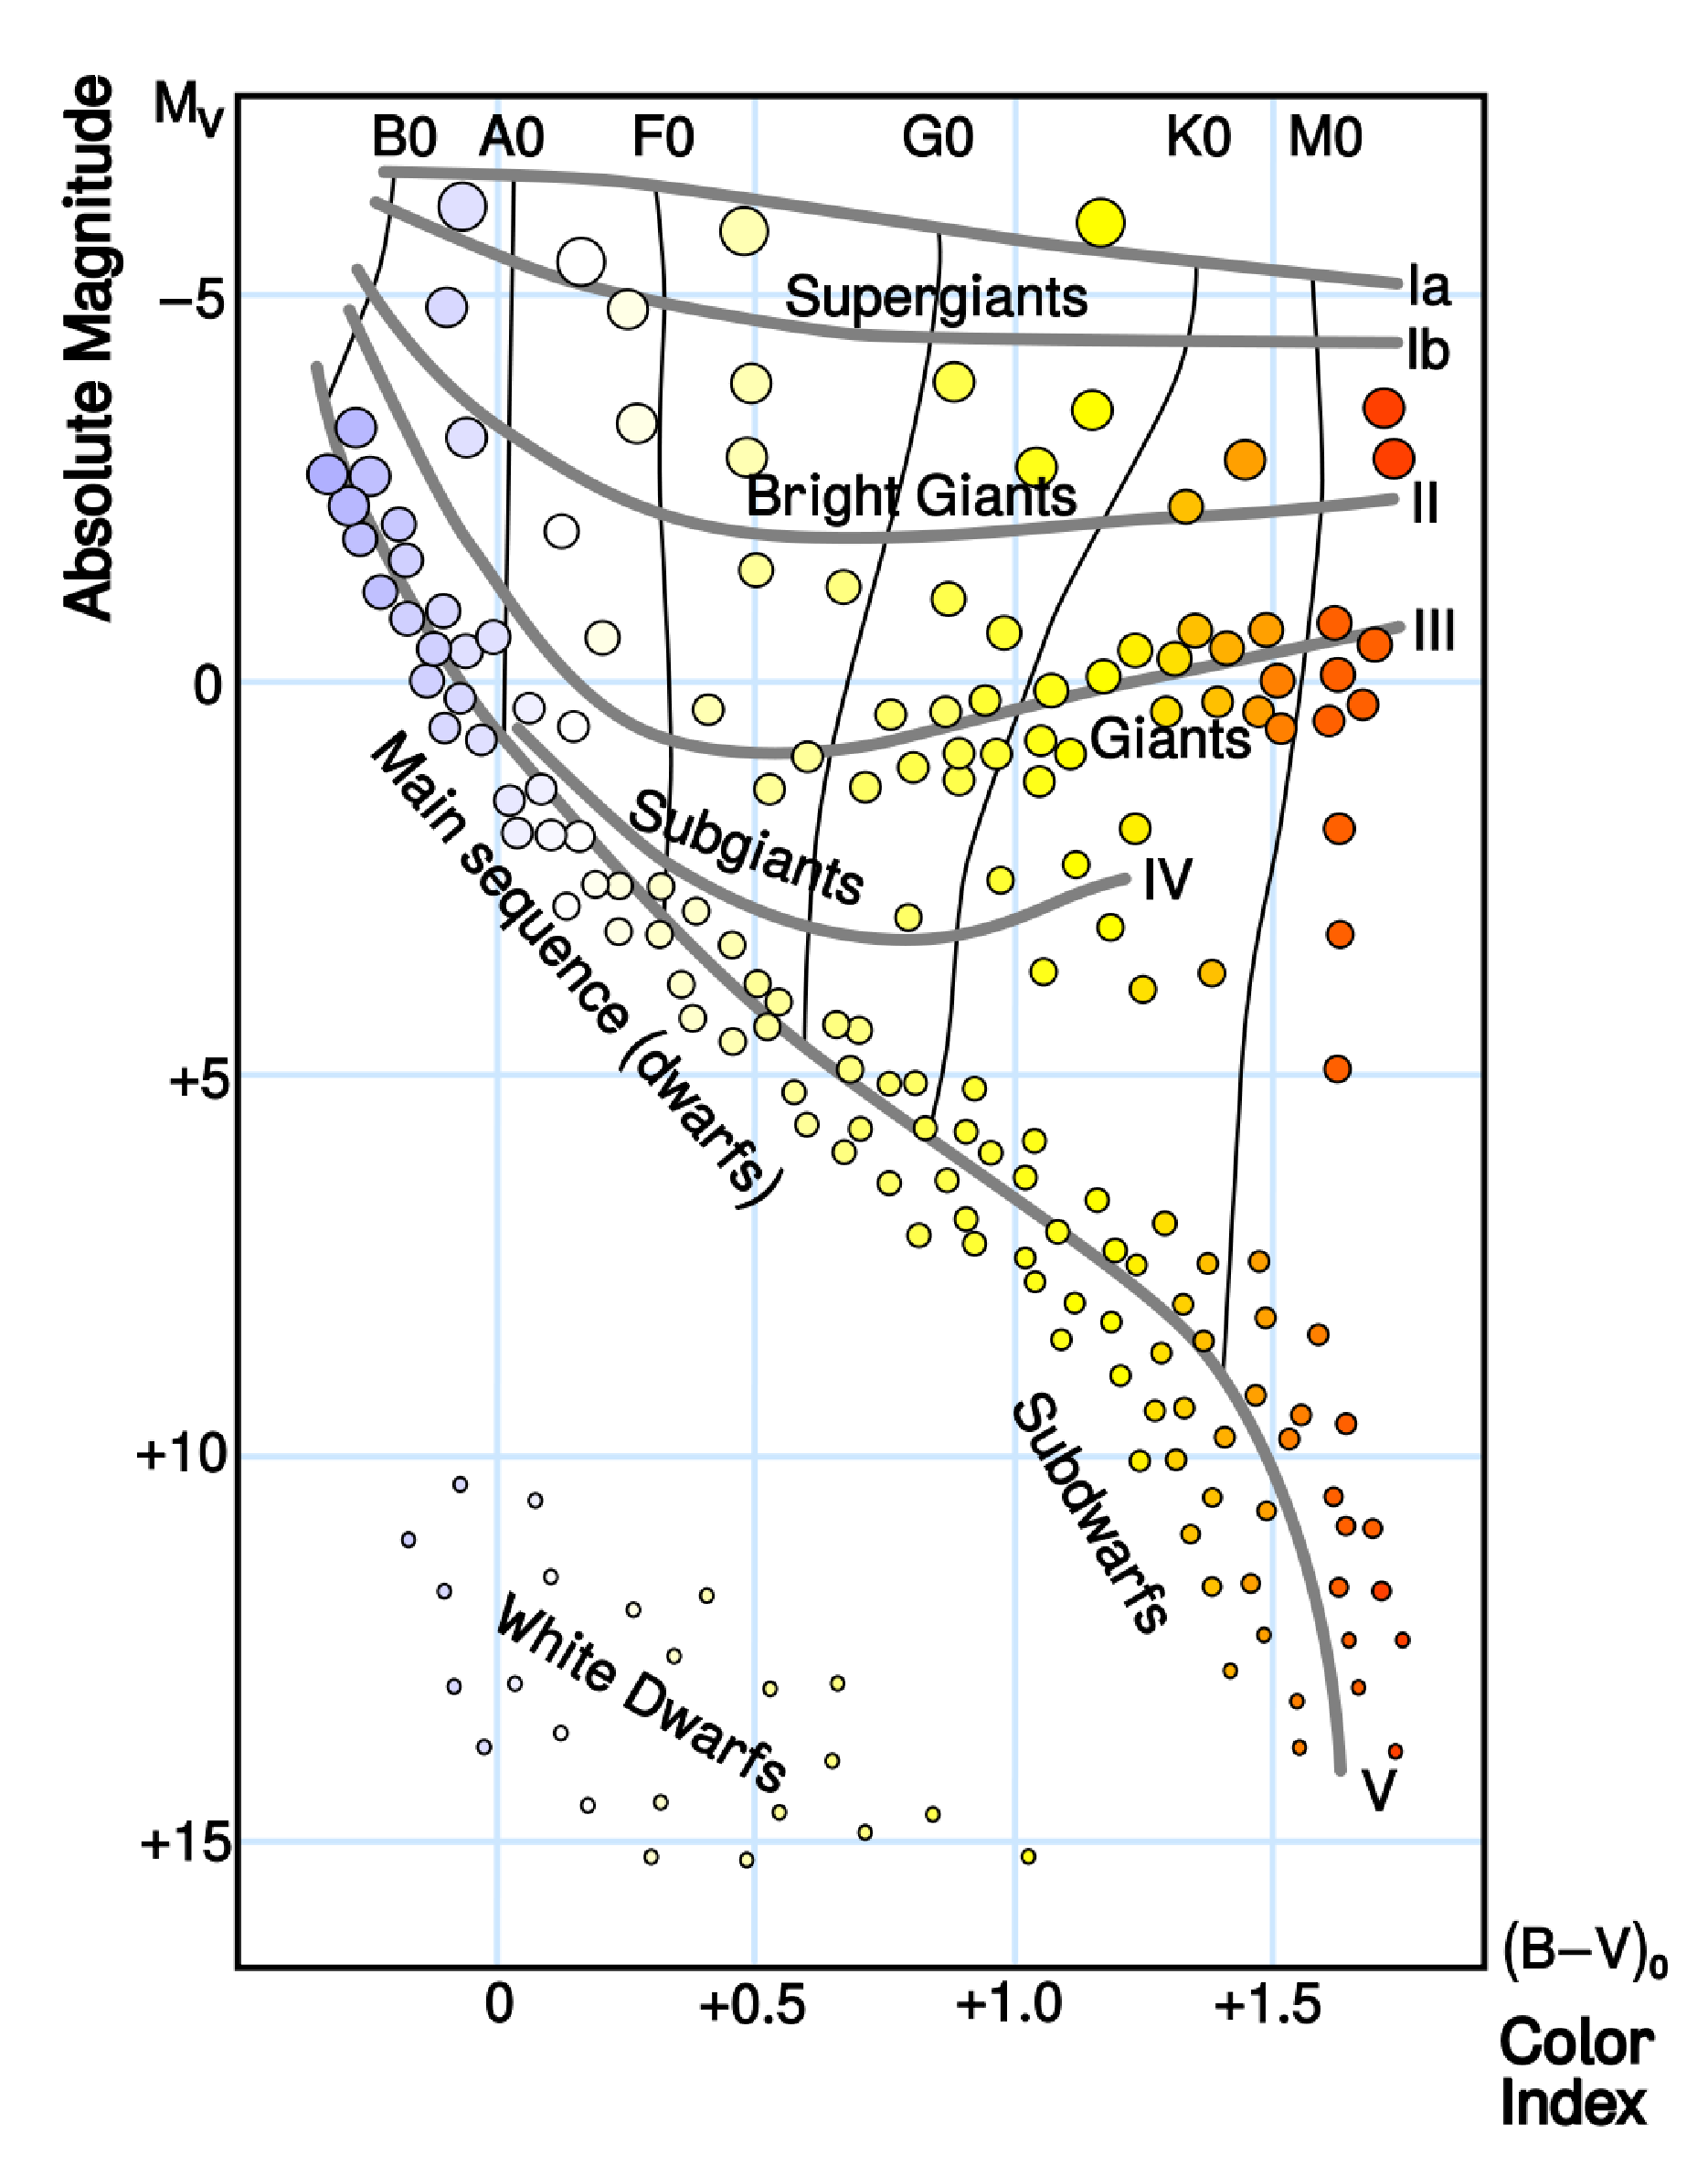
\includegraphics[scale=0.7]{H-R_diagram}%
\caption{The Hertzsprung-Russel diagram.}\label{fig:hertzsprung}
\end{center}\end{figure}

\begin{shaded}
\textbf{Exercise \theExercise \stepcounter{Exercise}} : Which of the following stars is the brightest? One with an absolute magnitude of -1 or one with a magnitude of +5. Explain your answer.\end{shaded}
\begin{shaded}
\textbf{Exercise \theExercise \stepcounter{Exercise}} : The colour of a star in the Hertzsprung-Russel diagram is represented by a colour-index, a number. A colour index of 0 means that the star's colour is blue, a red star has an index of 1.5. When you look at the diagram of figure~\ref{fig:hertzsprung} you can see different `groups'. The most pronounced group is the one running from the top left of the graph to the bottom right. This is the main sequence of dwarf (and sub-dwarf) stars. Can you explain why these stars are grouped along this diagonal line?\\ \textit{Hints: What influence does the size of a star have on its temperature? And what is the relationship between temperature and colour? To find an answer to the last question you might want to look up `Black-body Radiation' or `'Planck's Law`.}\end{shaded}

The absolute magnitude of a star can be found (calculated) by correcting the apparent magnitude for distance. The further you are removed from a light source the dimmer it seems to be: A candle at arms length is much brighter than all the stars in the night sky.

How can we correct for the distance of a light source? First let us take a look at \emph{how} distance influences the apparent magnitude or brightness. Imagine a light source in the centre of a box with sides of 1 metre. Every side of the box has a surface area of 1~m$^2$, so the total surface area of the box is 6~m$^2$. The light of the source is spread out over this surface. If we placed the light source in a box with sides 2 metres long, the same amount of light would have been spread out over a surface of 24~m$^2$. The average intensity of the light would be just 1/4 of what is was in the previous box ($\frac{6}{24}=\frac{1}{4}$). This means that by increasing the distance with a factor of 2, the light intensity decreases by a factor of 4 ($2^2$). The intensity of light follows a square law: \\
\indent \textbf{The apparent magnitude is inversely proportional to the distance squared.}\footnote{Or more concise: Apparent magnitude follows the inverse square law.}

\begin{shaded}
\textbf{Exercise \theExercise \stepcounter{Exercise}} : Lets test by reasoning if the apparent magnitude really follows the statement above. What happens to the average intensity of the light on the surface of the box when we increase the sides to 3, 4, or 5 metres. How would you argue that the statement is true for all lengths and that is not a mere coincidence that it holds for the chosen lengths?\end{shaded}

\end{document}
